\documentclass[times, utf8, seminar]{fit}

\usepackage{listings}
\usepackage{longtable}
\usepackage{xcolor}
\usepackage{float}
\usepackage{enumitem}
\usepackage{hyperref}
\usepackage{enumerate}
\usepackage{graphicx}
\usepackage{etoolbox}
\usepackage{datetime}
\usepackage{needspace}
\usepackage[compact]{titlesec}
\usepackage{setspace}
\onehalfspacing

\begin{document}
\widowpenalty=300
\clubpenalty=300

\lstset{
  language=bash,
  backgroundcolor=\color{gray!25},
  basicstyle=\ttfamily \footnotesize,
  breaklines=true,
  prebreak=\raisebox{0ex}[0ex][0ex] {\ensuremath{\hookleftarrow}},
  columns=fullflexible,
  keywords={},
  mathescape=false
}

\title{Agilni \emph{software development},\newline \emph{test} \& \emph{deployment}}

\author{Ernad Husremović}
\brindex{DL 2792}
\verzija {0.9.0}

\mentor{mr. Adil Joldić}

\maketitle

\tableofcontents

%\listoftables
%\listoffigures
\newpage

\begin{abstract}

U ovom radu se na bazi konkretnog primjera\footnote{"HOWTO" stil} prezentuje infrastruktura za testiranje i instalaciju u produkcijskom okruženju (''test'' \& ''deploy'' infrastructure). Obradićemo instalaciju ''Gitlab'' servera koristeći sljedeće tehnologije i servise:
\begin{itemize}
  \item Github/git \url{https://github.com/hernad/gitlabhq}
  \item Vagrant  \url{http://vagrantup.com/}
  \item Chef opscode \url{http://www.opscode.com/chef}
  \item Rackspace cloud \url{http://www.rackspace.com/cloud}
\end{itemize}

\keywords{open source software, OSS, chef, vagrant, rackspace, git, github}
\end{abstract}

% abstract end

\begin{document}
\setlength{\parindent}{0pt}


\chapter{Uvod}

%\vspace*{-1.2cm}
\section{\emph{Gitlab} projekat \emph{case study}}
Gitlab je web servis koji obezbjeđuje upravljanje softverskim projektima. Gitlab obezbjeđuje sljedeće funkcije:
\begin{itemize}
  \item Git source code management - hostiranje izvornog koda unutar git repozitorija
  \item Issue management - elektronsko praćenje aktivnosti developera
  \item Milestone management - pojedine aktivnosti (issues) se mogu vezati uz odgovarajuću verziju (iteraciju) - ''milestone''
  \item Code snippets (code templates) - publikovanje uzoraka izvornog koda koje će tim koristiti
  \item Code/Commit review - komentarisanje izvornog koda
  \item Wikies - wikiji omogućavaju timski razvoj projektne dokumentacije
\end{itemize}

\section{\emph{Gitlab} arhitektura}
''Gitlab'' je složen softverski sistem sastaljen od sljedećih komponenti:
\begin{enumerate}
  \item ubuntu linux server
  \item openssh server za razmjenu git repozitorija putem ssh protokola 
  \item ''nginx'' web server
  \item ''postfix'' email server
  \item ''ruby on rails'' framework je korišten za izradu web front-end-a.
  \item ''resque'' za background jobs \url{https://github.com/defunkt/resque}
  \item ''redis'' nosql (koristi ga ''resque'')
  \item ''mysql'' database backend\footnote{može se koristiti i postgresql}
  \item ''gitolite'' perl za upravljanje git repozitorijima
  \item ''pygments'' python ''source code higlighter''
\end{enumerate}

\section{\emph{Devops} metode}
Instalacija ovako složene infrastruktura traži značajno vrijeme i resurse za postavljanje, kako testnog tako i produkcijskog okruženja. 
Agilni pristup potencira mogućnost brzih promjena softverskog sistema. Konvencionalne metode instalacije i održavanja (manuelne procedure) su u slučajevima ovako kompleksnih sistema neadekvatne u tom konktekstu. Agilni pristup ovom problemu potencira automatizaciju testnog i produkcijskog okruženja. Manuelne operacije se zamjenjuju atomatiziranim procedurama. Operacije instalacije i održavanja sistema i same postaoju sofverski projekti.
Agilnog pristupa ovoj tematici je rezultirao ''Devops''\footnote{\url{http://en.wikipedia.org/wiki/DevOps}} metodama i praksama instalacije.

\chapter{Testno okruženje}
\section{\emph{Vagrant}}

''Chef'' je klasičan primjer ''devops'' alata. ''Chef'' recepti (''cookies'') sadrže programe kojim se instaliraju pojedine komponente sistema. Skup tih recepata definiše instalacijsku proceduru.

Naravno, produkcijskoj instalaciji sistema\footnote{instalaciji sistema namjenjenoj krajnjem kurisniku} predhodi testiranje.
''Vagrant'' je popularni alat koji su mnogi ''devops'' pobornici prihvatili kao alat za izgradnju testnog okruženja. 
''Vagrant'' za automatizaciju koristi ''Virtual Box'' virtuelne sesije\footnote{\url{https://www.virtualbox.org}}. Konfiguracija tih sesija se vrši sa ''chef configuration management'' sistemom\footnote{može da se koristi i ''Puppet'' configuration managment sistem}.

\section{Instalacija testnog gitlab servera}
\setlength{\parindent 0cm}

Preuzmimo vagrant\_gitlab projekat sa Github-a:

\$ \verb+git clone git://github.com/hernad/vagrant_gitlab.git+

Install skripta instalira sve potrebne ruby pakete koje će vagrant koristi\footnote{Naravno, prije toga je potrebno imati instalirano ''ruby'' programsko okruženje, preporučeno ''rvm'' ruby okruženje}, kao i sve ''cookbooks'' koje će koristiti ''chef'':

vagrant\_gitlab\$ \verb+./install.sh+

Vagrantfile\footnote{\url{https://github.com/hernad/vagrant\_gitlab/blob/master/Vagrantfile}} sadrži konfiguraciju testnog gitlab servera. Vagrantfile nije ništa drugo nego ''ruby'' program. Konkretno, vagrant\_gitlab koristi niz sistemskih varijabli (OS environment)  kao parametre instalacije sistema\footnote{Parametri sadrže sve ono što su privatni podaci korisnika i što ne treba biti javno dostupno - imena hostova, korisnika, lozinke i sl.}

Komandom \verb+up.sh+ setujemo sistemske varijable, te kreiramo virutelnu sesiju:

vagrant\_gitlab\$ \verb+source up.sh+

\begin{lstlisting}
OS_AUTH_SYSTEM=rackspace
OS_AUTH_URL=https://identity.api.rackspacecloud.com/v2.0/
OS_DNS_DOMAIN=test.out.ba
OS_ENVARS='GMAIL_USER=bring.out.sa@gmail.com GMAIL_PASSWORD=pwd1 MYSQL_ROOT_PWD=pwd2 MYSQL_PWD=pwd3 GITHUB_USER=hernad GITHUB_PROJECT=vagrant_gitlab OS_SERVER_NAME=gitlab-stable.test.out.ba OS_DNS_DOMAIN=test.out.ba GITLAB_VERSION=v3.0.2 GITLAB_REPOS=git://github.com/hernad/gitlabhq.git'
OS_NO_CACHE=1
OS_PASSWORD=<rackspacecloud_api_key>
OS_PROJECT_ID=<rackspace_user>
...
\end{lstlisting}

Nakon kreiranja gitlab ''VirtualBox'' testne sesije, slijedi pokretanje ''chef-solo'' procesa unutar sesije. ''chef-solo''\footnote{Chef-solo koristi lokalno instalirane ''cookbooks''. Standardna opcija je client-server, u kojoj chef agent (klijent) koji sa centralog chef-servera uzima ''cookbooks''} je zadužen za instalaciju i konfiguraciju testne sesije:

vagrant\_gitlab\$ \verb+source ./up.sh+
\begin{lstlisting}
[default] Clearing any previously set forwarded ports...
[default] Forwarding ports...
[default] -- 22 => 2222 (adapter 1)
[default] Creating shared folders metadata...
...
[default] Waiting for VM to boot. This can take a few minutes. <<<<<<< virtualbox sesija kreirana
[default] VM booted and ready for use!
[default] Detected Virtualbox Guest Additions 4.2.4 --- OK.
[default] Configuring and enabling network interfaces...
[default] Mounting shared folders...
[default] -- v-root: /vagrant
[default] -- v-csc-1: /tmp/vagrant-chef-1/chef-solo-1/cookbooks
[default] Running provisioner: Vagrant::Provisioners::ChefSolo...
[default] Generating chef JSON and uploading...
[default] Running chef-solo... <<<<<<<<<<< Pokrece se chef-solo na virtualbox sesiji
stdin: is not a tty
[Mon, 19 Nov 2012 11:33:15 +0000] INFO: *** Chef 0.10.10 ***
[Mon, 19 Nov 2012 11:33:15 +0000] INFO: Setting the run_list to ["recipe[build-essential]", "recipe[rvm::system]", "recipe[mysql::client]", "recipe[mysql::ruby]", "recipe[postgresql::client]", "recipe[postgresql::ruby]", "recipe[gitlab::default]", "recipe[gitlab::nginx]", "recipe[gitlab::database]"] from JSON
[Mon, 19 Nov 2012 11:33:15 +0000] INFO: Run List is [recipe[build-essential], recipe[rvm::system], recipe[mysql::client], recipe[mysql::ruby], recipe[postgresql::client], recipe[postgresql::ruby], recipe[gitlab::default], recipe[gitlab::nginx], recipe[gitlab::database]]
[Mon, 19 Nov 2012 11:33:15 +0000] INFO: Run List expands to [build-essential, rvm::system, mysql::client, mysql::ruby, postgresql::client, postgresql::ruby, gitlab::default, gitlab::nginx, gitlab::database]
[Mon, 19 Nov 2012 11:33:15 +0000] INFO: Starting Chef Run for precise32
...
[Mon, 19 Nov 2012 11:36:20 +0000] INFO: Processing package[ssl-cert] action install (/tmp/vagrant-chef-1/chef-solo-1/cookbooks/rvm/providers/ruby.rb line 156)
[Mon, 19 Nov 2012 11:36:22 +0000] INFO: package[ssl-cert] installed version 1.0.28ubuntu0.1
[Mon, 19 Nov 2012 11:36:22 +0000] INFO: Building rvm_ruby[ruby-1.9.3-p327], this could take awhile...
...
[Mon, 19 Nov 2012 14:18:58 +0000] INFO: Processing service[nginx] action reload (nginx::default line 39)
[Mon, 19 Nov 2012 14:18:58 +0000] INFO: service[nginx] reloaded
[Mon, 19 Nov 2012 14:18:58 +0000] INFO: template[/etc/init.d/gitlab] sending enable action to service[gitlab] (delayed)
[Mon, 19 Nov 2012 14:18:58 +0000] INFO: Processing service[gitlab] action enable (gitlab::default line 183)
[Mon, 19 Nov 2012 14:18:58 +0000] INFO: Chef Run complete in 994.730999 seconds
[Mon, 19 Nov 2012 14:18:58 +0000] INFO: Running report handlers
[Mon, 19 Nov 2012 14:18:58 +0000] INFO: Report handlers complete
\end{lstlisting}

Nakon 15-tak minuta imamo u potpunosti instaliran ''gitlab'' server.

\section{\emph{Chef cookbooks} - knjige recepata za instalaciju sistema}

\subsection{Opscode standardni cookbook - mysql}
Veliki broj ''chef'' knjiga recepata već postoji spreman. Uzmimo primjer msysql\footnote{\url{http://community.opscode.com/cookbooks/mysql}} cookbook-a.
Sve što je potrebno jesu tri jednostavna koraka:
\begin{enumerate}
  \item \href{https://github.com/hernad/vagrant_gitlab/blob/1054da0674f9/Cheffile#L14}{\color{blue}{Uvrsti mysql cookbook}} u knjigu recepata koje gitlab projekat koristi
  \item Uključi ''recipe'' u \href{https://github.com/hernad/vagrant_gitlab/blob/1054da0674f9fa586/Vagrantfile#L18}{\color{blue}{Vagrantfile}}
  \item Definiši \href{https://github.com/hernad/vagrant_gitlab/blob/b2fbc3391822e75c5/Vagrantfile#L66}{\color{blue}{parametre instalacije}}
\end{enumerate}

\subsection{Projektni cookbook - gitlab}

Za potrebe našeg projekta pravimo sopstveni cookbook\footnote{\url{https://github.com/hernad/chef_gitlab}} (ili više njih, vodeći se ''reusable'' principima).

Unutar njega koristimo komande iz standardnih cookbook-ova, kao što je gore navedeni \href{https://github.com/hernad/chef_gitlab/blob/5d04c1885d9cc37/recipes/database.rb#L54}{mysql} ili jednostavno navodimo operacije koje su potrebne za instalaciju i konfiguraciju naše aplikacije.

\subsection{\emph{Cookbook} principi}

Kod izrade cookbook-a treba imati na umu sljedeće principe:
\begin{itemize}
  \item Idempotentnost - cookbook se može bez problema pokrenuti više puta, ishod instalacije treba biti ''identičan'' 
  \item Multi-environment pristup - predvidjeti sva ciljna okruženja (testno/produkcijsko, operativni sistemi, ciljni servis provajderi). Tehnički, ovaj princip se realizira parametrizacijom
  \item Parametrizacija - Svi parametri sistema koji su predmet promjena prilikom različitih scenarija instalacije treba parametrizirati.
\end{itemize}

\chapter{\emph{Git} i \emph{chef}}

U ovom poglavlju ćemo demonstrirati efekte pravilne parametrizacije ''cookbook''-ova. Takođe ćemo deminstrirati  korištenje git repozitorija unutar chef recepata. ''Chef'', treba li to uopšte naglasiti, ima odličnu podršku za git repozitorije. 

\section{Gitlab ''merge'' from upstream}
Ključni sofware repozitorij je naravno izvorni kod same gitlab aplikacije \url{https://github.com/hernad/gitlabhq}.
Ovaj repozitorij predstavlja ''fork'' glavnog - ''upstream'' projekta.

\begin{figure}[H]
\centering
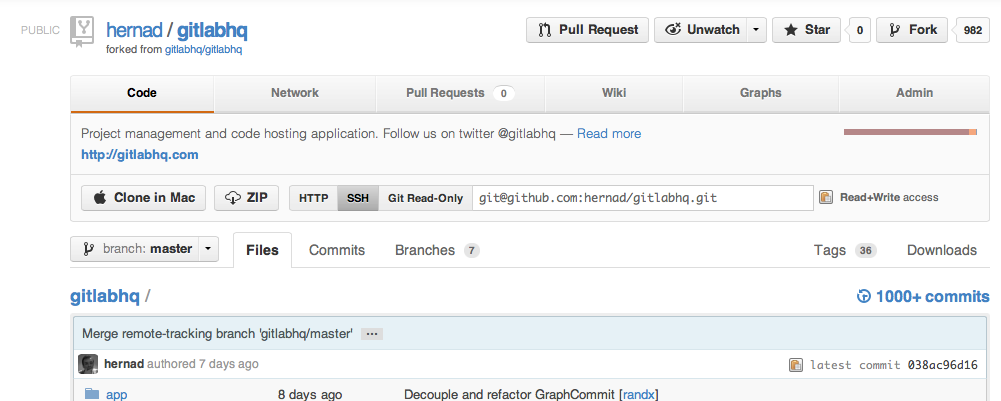
\includegraphics[width=15cm]{img/gitlabhq_hernad_fork.png}
\caption{Fork ''gitlabhq'' od strane developera ''hernad}
\end{figure}

Glavni (''upstream'') repozitorij projekta nalazi se na \url{https://github.com/gitlabhq/gitlabhq}.

\begin{figure}[H]
\centering
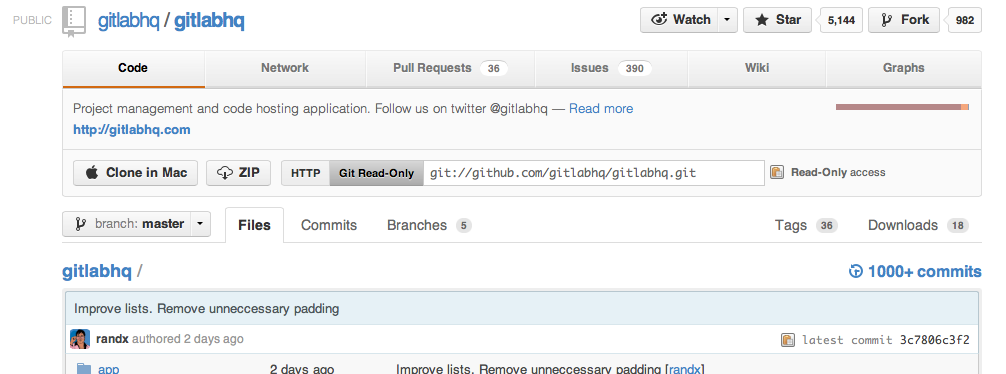
\includegraphics[width=15cm]{img/gitlabhq_upstream.png}
\caption{Gitlabhq ''upstream'' projekat}
\end{figure}

Git ''merge proces'' omogućava spajanje različitih branch-ova unutar jednog ili više git repozitorija\citep{agilegit}
Definišimo lokaciju upstream repozitorija:

gitlabhq\$ \newline\verb+git remote add gitlabhq git://github.com/gitlabhq/gitlabhq.git+

Preuzmimo promjene sa upstream-a:

gitlabhq\$ \verb+git fetch gitlabhq+
\begin{lstlisting}
remote: Counting objects: 570, done.
remote: Compressing objects: 100\% (174/174), done.
remote: Total 342 (delta 262), reused 237 (delta 165)
Receiving objects: 100\% (342/342), 43.70 KiB, done.
Resolving deltas: 100\% (262/262), completed with 122 local objects.
From git://github.com/gitlabhq/gitlabhq
   dd4d124..3c7806c  master     -> gitlabhq/master
\end{lstlisting}

Pogledajmo koji je naš trenutni branch:

gitlabhq\$ \verb+git branch -l+
\begin{lstlisting}
* master
\end{lstlisting}

\begin{figure}[H]
\centering
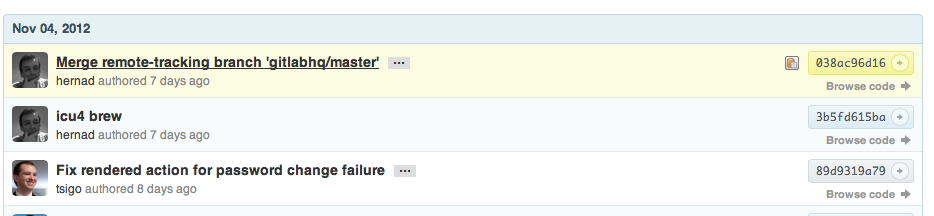
\includegraphics[width=15cm]{img/gitlabhq_hernad_prije_merge.png}
\caption{''gitlabhq'' repozitorij - hernad fork prije merge operacije}
\end{figure}


Naš lokalni branch ne sadrži promjene koje su na ''upstream'' projektu rađene posljednjih par dana. ''Merge'' operacijom te promjene ubacujemo u naš repozitorij:

gitlabhq\$ \verb+git merge gitlabhq/master+
\begin{lstlisting}
Removing lib/gitlab/encode.rb
Removing gitlab
Auto-merging doc/development.md
Removing Procfile.production
Merge made by the recursive strategy
 .travis.yml                                        |    2 +-
 CHANGELOG                                          |    2 +-
 ....
 VERSION                                            |    2 +-
 app/assets/images/event_filter_comments.png        |  Bin 0 -> 750 bytes
 app/assets/images/event_filter_merged.png          |  Bin 0 -> 463 bytes
 app/assets/images/event_filter_push.png            |  Bin 0 -> 632 bytes
 ...
 app/controllers/application_controller.rb          |    9 +++
 app/controllers/blob_controller.rb                 |   10 +--
 app/controllers/dashboard_controller.rb            |   11 ++-
 app/controllers/profile_controller.rb              |    2 +-
 ...
 app/views/blame/show.html.haml                     |    4 +-
 app/views/commits/_commit.html.haml                |    4 +-
 app/views/commits/_head.html.haml                  |    5 ++
 app/views/dashboard/index.html.haml                |    9 ++-
 
 ... 
 
 delete mode 100644 Procfile.production
 create mode 100644 app/assets/images/event_filter_comments.png
 create mode 100644 app/assets/images/event_filter_merged.png
 ...
 delete mode 100644 lib/gitlab/encode.rb
 create mode 100644 lib/gitlab/git_stats.rb
 create mode 100644 vendor/assets/javascripts/g.bar-min.js
 create mode 100644 vendor/assets/javascripts/g.raphael-min.js
\end{lstlisting}

Nije bilo nikakvih konflikata, tako da je automatsko merdžiranje bilo dovoljno. U slučaju konflikata, moralo bi se obaviti ručno spajanje fjalova koji su u konfliktu\footnote{Npr. ako se i na ''hernad'' fork objektu radilo na nekom source fajlu, git prijavljuje konflikt i upućuje na ručne ispravke tog fajla da bi se merdžiranje završilo}.

Pushiramo promjene na ''origin'' remote lokaciju, što je ustvari fork repozitorij githab-a developera ''hernad'': 
gitlabhq\$ \verb+git push origin master+

\begin{lstlisting}
Counting objects: 581, done.
Delta compression using up to 8 threads.
Compressing objects: 100\% (85/85), done.
Writing objects: 100\% (350/350), 45.00 KiB, done.
Total 350 (delta 267), reused 342 (delta 262)
To git@github.com:hernad/gitlabhq.git
   038ac96..28f5807  master -> master
\end{lstlisting}

\section{Instalacija različitih verzija gitlab-a}

Kod izgradnje ''gitlab'' cookbook-a su predviđeni paramteri \href{https://github.com/hernad/chef_gitlab/blob/master/attributes/default.rb#L9}{\color{blue}{''gitlab\_url'' i ''gitlab\_branch''}}. Unutar Vagrantfile-a se ti parametri popunjavaju sa varijablama GITLAB\_VERSION i GITLAB\_REPOS.

One su ugniježđene u OS envar ''OS\_ENVARS''\footnote{Ovo ''ugnježđivanje'' je napravljeno iz tehničkih razloga. Naime ti parametri nam trebaju biti dostupni i kod instalacije udaljenog produkcijskog servera (Instalacija na rackspace cloud).}.

Definišimo instalaciju verzije 3.0.2\footnote{U repozitoriju se nalazi git tag ''v3.0.2''}, sa repozitorija ''hernad'':
\begin{lstlisting}
OS_ENVARS='... GITLAB_VERSION=v3.0.2 GITLAB_REPOS=git://github.com/hernad/gitlabhq.git'
\end{lstlisting}

Rezultat će biti instalacija verzije 3.0.2 gitlab aplikacije na ciljni server. Ako želimo instalirati posljednju verziju, jednostavno navodimo \verb+GITLAB_VERSION=master+. Na taj način možemo na testni server instalirati posljednju verziju, a na produkcijski poseljednju stabilnu verziju (npr. v3.0.2):

\begin{figure}[H]
\centering
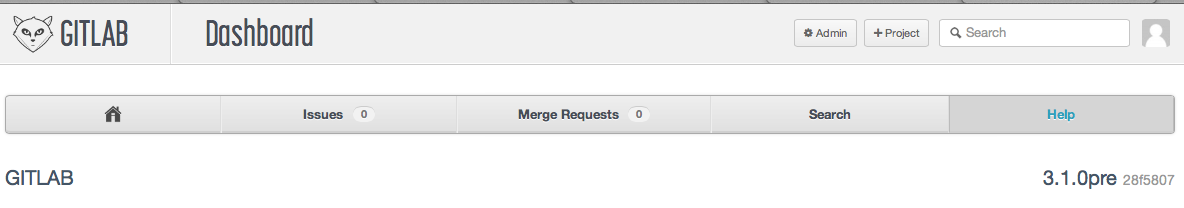
\includegraphics[width=15cm]{img/gitlab_hernad_310_after_merge.png}
\caption{Gitlabhq nakon `merge' operacije sa `upstream' projektom - ''master'' branch je verzija 3.1.0-pre}
\end{figure}

\chapter{Instalacija na produkcijski server}

Jednostavna uspostava testnog okruženja uz pomoć Vagrant-a je bitna stvar. Međutim, ako se produkcijsko okruženje mora uspostaviti manuelno, nismo dobili previše na agilnosti.

Dobra je stvar da se ''Chef'' može primijeniti i na ''produkcijsko'' okruženje bez ikakvih značajnih intervencija.

\section{Rackspace \emph{cloud}}

Mi ćemo za produkcijsko okruženje koristiti rackspace cloud:

\begin{figure}[H]
\centering
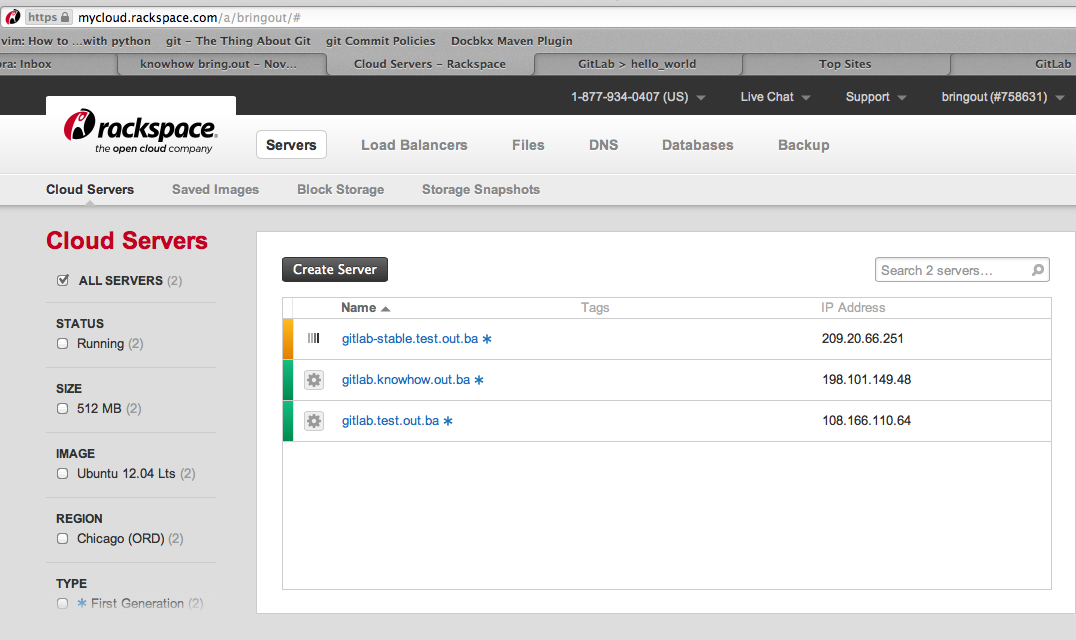
\includegraphics[width=15cm]{img/rackspace_servers.png}
\caption{Rackspace cloud web upravljačka konzola}
\end{figure}

''Rackspace'' je odabran zato što postoji kvalitetan developerski API\footnote{\url{http://docs.rackspace.com/api/}} za upravljanje svim cloud resursima. ''Chef'' recepti nas vode korak do potpune automatske instalacije produkcijskog servera. 

\section{\emph{Bootstrap} i instalacija rackspace servera}

U odnosu na naše ''Vagrant'' testno okruženje trebamo sljedeće nove funkcije:
\begin{itemize}
  \item Kreirati rackspace server 
  \item Instalirati na njega chef radno okruženje\footnote{\url{https://github.com/hernad/ubuntu_bootstrap_chef/blob/master/bootstrap.sh}}
  \item Pokrenuti željene chef cookbooks, sa zadanim parametrima (OS\_ENVARS)\footnote{\url{https://github.com/hernad/ubuntu_bootstrap_chef/blob/master/run_solo.sh}}
  \item Registrovati novokreirani server na rackspace DNS sistemu\footnote{\url{https://github.com/hernad/ubuntu_bootstrap_chef/blob/master/rackspace/manage_domains.py}}
\end{itemize}

Sve ove funkcije realizira ''ubuntu\_bootstrap\_chef''\footnote{\url{https://github.com/hernad/ubuntu_bootstrap_chef}} projekat.

Komanda \href{https://github.com/hernad/ubuntu\_bootstrap\_chef/blob/master/rackspace/setup\_rack\_server.sh}{\color{blue}{setup\_rack\_server}} u jednom koraku realizira sve gornje korake:

\begin{lstlisting}
Server: gitlab.knowhow.out.ba IP: 198.101.149.48
vrsim update domena knowhow.out.ba, zapis gitlab.knowhow.out.ba sa javnom adresom 198.101.149.48
./manage_domains.py -d knowhow.out.ba -r gitlab.knowhow.out.ba -i 198.101.149.48
dns_domain: knowhow.out.ba dns_record: gitlab.knowhow.out.ba ip_address 198.101.149.48

....

[2012-11-12T11:15:43+00:00] INFO: template[/etc/rvmrc] mode changed to 644
[2012-11-12T11:15:43+00:00] INFO: Processing execute[install system-wide RVM] action run (rvm::system_install line 76)
[2012-11-12T11:15:43+00:00] INFO: Processing execute[upgrade system-wide RVM to none] action run (rvm::system_install line 110)
[2012-11-12T11:15:43+00:00] INFO: Processing rvm_ruby[ruby-1.9.3-p327] action install (rvm::system line 170)
/root/vagrant_gitlab/cookbooks/rvm/libraries/rvm_chef_user_environment.rb:36: warning: class variable access from toplevel
[2012-11-12T11:15:45+00:00] INFO: Processing package[build-essential] action install (/root/vagrant_gitlab/cookbooks/rvm/providers/ruby.rb line 156)
[2012-11-12T11:15:45+00:00] INFO: Processing package[openssl] action install (/root/vagrant_gitlab/cookbooks/rvm/providers/ruby.rb line 156)
[2012-11-12T11:15:45+00:00] INFO: Processing package[libreadline6] action install (/root/vagrant_gitlab/cookbooks/rvm/providers/ruby.rb line 156)
[2012-11-12T11:15:45+00:00] INFO: Processing package[libreadline6-dev] action install (/root/vagrant_gitlab/cookbooks/rvm/providers/ruby.rb line 156)
[2012-11-12T11:15:45+00:00] INFO: Processing package[zlib1g] action install (/root/vagrant_gitlab/cookbooks/rvm/providers/ruby.rb line 156)
[2012-11-12T11:15:45+00:00] INFO: Processing package[zlib1g-dev] action install (/root/vagrant_gitlab/cookbooks/rvm/providers/ruby.rb line 156)
[2012-11-12T11:15:45+00:00] INFO: Processing package[libssl-dev] action install (/root/vagrant_gitlab/cookbooks/rvm/providers/ruby.rb line 156)
[2012-11-12T11:15:45+00:00] INFO: Processing package[libyaml-dev] action install (/root/vagrant_gitlab/cookbooks/rvm/providers/ruby.rb line 156)

...

[2012-11-12T11:15:45+00:00] INFO: Processing package[libsqlite3-dev] action install (/root/vagrant_gitlab/cookbooks/rvm/providers/ruby.rb line 156)
[2012-11-12T11:15:45+00:00] INFO: Processing package[sqlite3] action install (/root/vagrant_gitlab/cookbooks/rvm/providers/ruby.rb line 156)
[2012-11-12T11:15:46+00:00] INFO: Processing package[libxml2-dev] action install (/root/vagrant_gitlab/cookbooks/rvm/providers/ruby.rb line 156)
[2012-11-12T11:15:46+00:00] INFO: Processing package[libxslt-dev] action install (/root/vagrant_gitlab/cookbooks/rvm/providers/ruby.rb line 156)
[2012-11-12T11:15:46+00:00] INFO: package[libxslt-dev] is a virtual package, actually acting on package[libxslt1-dev]
[2012-11-12T11:15:46+00:00] INFO: Processing package[autoconf] action install (/root/vagrant_gitlab/cookbooks/rvm/providers/ruby.rb line 156)
[2012-11-12T11:15:46+00:00] INFO: Processing package[libc6-dev] action install (/root/vagrant_gitlab/cookbooks/rvm/providers/ruby.rb line 156)
[2012-11-12T11:15:46+00:00] INFO: Processing package[ncurses-dev] action install (/root/vagrant_gitlab/cookbooks/rvm/providers/ruby.rb line 156)
[2012-11-12T11:15:46+00:00] INFO: package[ncurses-dev] is a virtual package, actually acting on package[libncurses5-dev]
[2012-11-12T11:15:46+00:00] INFO: Processing package[automake] action install (/root/vagrant_gitlab/cookbooks/rvm/providers/ruby.rb line 156)
[2012-11-12T11:15:46+00:00] INFO: Processing package[libtool] action install (/root/vagrant_gitlab/cookbooks/rvm/providers/ruby.rb line 156)
[2012-11-12T11:15:46+00:00] INFO: Processing package[bison] action install (/root/vagrant_gitlab/cookbooks/rvm/providers/ruby.rb line 156)
[2012-11-12T11:15:46+00:00] INFO: Processing package[ssl-cert] action install (/root/vagrant_gitlab/cookbooks/rvm/providers/ruby.rb line 156)
[2012-11-12T11:15:47+00:00] INFO: Building rvm_ruby[ruby-1.9.3-p327], this could take awhile...

....

boostrap chef for vagrant_gitlab is finished (0.9.9) :)
restartujem server ...
Restartujem server gitlab.knowhow.out.ba

real15m29.472s
user0m3.928s
sys0m0.387s
\end{lstlisting}

Nakon 30-tak minuta naš novokreirani rackspace server je konfigurisan i spreman da odmah obrađuje zahtjeve internet korisnika !

\subsection{Kako \emph{bootstrap} funkcioniše}

Generalno, boostrap projekat nakon isntalacije servera preuzima cookbooks iz projekta zadanog parametrom \verb+GITHUB_PROJECT=vagrant_gitlab+.
To znači da je ova procedura primjenljiva i na različite projekte (npr. \verb+GITHUB_PROJECT=vagrant_redmine+), naravno pod uslovom da se u njima obezbjedi sadržaj i struktura kakvu boostrap okruženje traži.  

U ''cookbook'' projektu se moraju nalaziti \href{https://github.com/hernad/vagrant_gitlab/blob/master/solo.rb}{\color{blue}{solo.rb}} i \href{https://github.com/hernad/vagrant_gitlab/blob/master/node.json}{\color{blue}{node.json}}. Oni imaju identičnu funkciju kakav ima Vagrantfile u testnoj instalaciji\footnote{Lahko je uočiti, da je \href{https://github.com/hernad/vagrant_gitlab/blob/master/roles/gitlab.rb}{\color{blue}{roles/gitlab.rb}} dobijen sa copy-paste sadržaja \href{https://github.com/hernad/vagrant_gitlab/blob/master/Vagrantfile}{\color{blue}{Vagrantfile-a}}}

\chapter{Zaključak}

\emph{Agilni} sofverski projekat je sposoban brzo reagovati na promjene\citep{agileart}.  Da bi to bilo moguće, agilnost se mora primjeniti u svim fazama životnog ciklusa softverskog projekta.

\emph{Devops} prakse i procedure su zadatke instalacije, konfiguracije i nadogradnje softverskog rješenja pretvorile u zasebne softverske projekte. Zadaci koji se pred sistemske inžinjere postavljaju kod instalacije \emph{cloud} infrastrukture daju agilnim metodama još veći značaj. 
Agilne \emph{devops} prakse su već sada ''must be'' pristup građenju IT sistema u \emph{cloud}-u. Treba imati na umu da ovaj koncept već sada ''ulazi'' i u konvencionalna IT odjeljenja. Brzi trend integracije privatne i javne cloud infrastrukture će bitnost ovog pristupa \emph{software deployment} operacijama još više uvećati.

% -------------------------------------------------
\bibliography{literatura}
\bibliographystyle{fit}

\appendix

\chapter{Gitlab \emph{cookbook} parametri}

Cookbook parametre možemo smjestiti u \verb+~/.bash_profille+. Primjer sadržaja:
\begin{lstlisting}
export OS_SERVER_NAME="gitlab-stable.test.out.ba"
export OS_DNS_DOMAIN="test.out.ba"

export GITLAB_REPOS="git://github.com/hernad/gitlabhq.git"
export GITLAB_VERSION="v3.0.3"

# OS_ENVARS sadrzi sve varijable koje chef-solo treba kod konifiguracije remote sistema
OS_ENVARS="GMAIL_USER=bring.out.sa@gmail.com GMAIL_PASSWORD=pwd_bring_sa"
OS_ENVARS="$OS_ENVARS MYSQL_ROOT_PWD=pwd_my_root MYSQL_PWD=pwd_my"
OS_ENVARS="$OS_ENVARS GITHUB_USER=hernad GITHUB_PROJECT=vagrant_gitlab"
OS_ENVARS="$OS_ENVARS OS_SERVER_NAME=$OS_SERVER_NAME OS_DNS_DOMAIN=$OS_DNS_DOMAIN"
OS_ENVARS="$OS_ENVARS GITLAB_VERSION=$GITLAB_VERSION GITLAB_REPOS=$GITLAB_REPOS"
export OS_ENVARS
\end{lstlisting}

Značenje parametara:
\begin{itemize}
  \item \verb+OS_SERVER_NAME+ - hostname servera
  \item \verb+OS_DNS_DOMAIN+ - pripadnost servera DNS domeni (koristi za automatski update rackspace DNS sistema}
  \item \verb+GITLAB_REPOS+, \verb+GITLAB_VERSION+ - git repozitorij ''gitlab'' projekta, verzija (branch, tag) koja se instalira
  \item \verb+GMAIL_USER+, \verb+GMAIL_PASSWORD+ - postfix email ser podešava za relaying prekod gmail-a
  \item \verb+GITHUB_USER+, \verb+GITHUB_PROJECT+ - odavde se preuzimaju cookbook-ovi
  \item \verb+MYSQL_ROOT_PWD+, \verb+MYSQL_PWD+ - root password mysql servera, password ''gitlab'' mysql usera 

\end{document}
